\documentclass[10pt]{standalone}
\usepackage[utf8]{inputenc}
\usepackage{pgf,tikz}
\usepackage{mathrsfs}
\usetikzlibrary{arrows}
\pagestyle{empty}
\usepackage[T1]{fontenc} % font encoding
\usepackage[utf8]{inputenc} % input encoding
%\usepackage{noto}
\usepackage[largesc]{newtxtext} %
\usepackage[varqu,varl]{zi4}% inconsolata
\usepackage{cabin}% sans serif
\usepackage[vvarbb]{newtxmath}
\useosf % use oldstyle figures except in math
\begin{document}
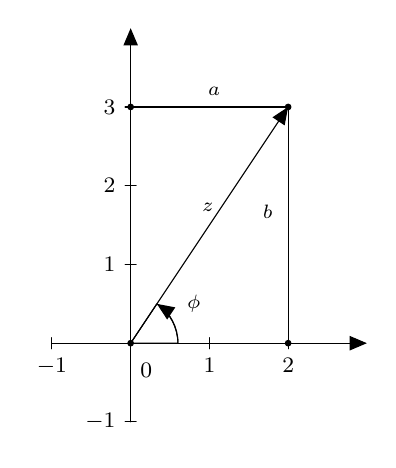
\begin{tikzpicture}[line cap=round,line join=round,>=triangle 45,x=1.0cm,y=1.0cm]
\draw[->,color=black] (-1.,0.) -- (3.,0.);
\foreach \x in {-1,1,2}
\draw[shift={(\x,0)},color=black] (0pt,2pt) -- (0pt,-2pt) node[below] {\footnotesize $\x$};
\draw[->,color=black] (0.,-1.) -- (0.,4.);
\foreach \y in {-1,1,2,3}
\draw[shift={(0,\y)},color=black] (2pt,0pt) -- (-2pt,0pt) node[left] {\footnotesize $\y$};
\draw (0pt,-10pt) node[right] {\footnotesize $0$};
\clip(-1.,-1.) rectangle (3.,4.);
\draw [shift={(0.,0.)}] (0,0) -- (0.:0.6) arc (0.:56.309932474020215:0.6) -- cycle;
\draw [->] (0.,0.) -- (2.,3.);
\draw [shift={(0.,0.)},->,color=black] (0.:0.6) arc (0.:56.309932474020215:0.6);
\draw  (2.,3.)-- (2.,0.);
\draw  (2.,3.)-- (0.,3.);
\begin{scriptsize}
\draw [fill=black] (2.,3.) circle (1.0pt);
\draw [fill=black] (0,0) circle (1.0pt);
\draw (0.98,1.73) node {$z$};
\draw [fill=black] (2.,0.) circle (1.0pt);
\draw (1.74,1.67) node {$b$};
\draw [fill=black] (0.,3.) circle (1.0pt);
\draw (1.06,3.2) node {$a$};
\draw (0.8,0.5) node {$\phi$};
\end{scriptsize}
\end{tikzpicture}
\end{document}